\usetikzlibrary{arrows.meta}
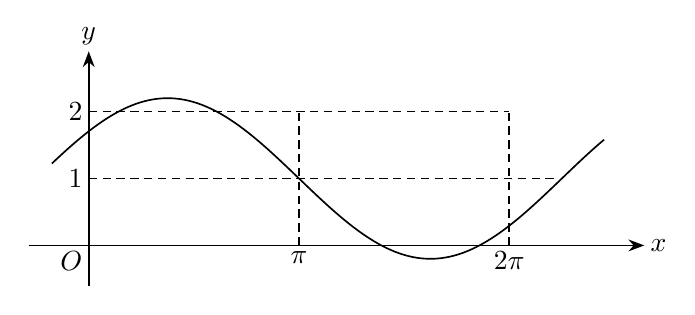
\begin{tikzpicture}[x=0.85cm,y=0.85cm,line width=.6pt,>=Stealth,font=\normalsize]
\draw[->] (-0.9,0)--(8.3,0) node[right,inner sep=0pt,xshift=2pt] {$x$};
\draw[->] (0,-0.6)--(0,2.9) node[above,inner sep=0pt,yshift=2pt] {$y$};
\node[below left,inner sep=0pt,xshift=-2pt,yshift=-2pt] at (0,0) {$O$};
\draw[densely dashed] (0,1)--(7.0,1);
\draw[densely dashed] (0,2)--(6.2832,2);
\draw[densely dashed] (3.1416,0)--(3.1416,2);
\draw[densely dashed] (6.2832,0)--(6.2832,2);
\draw[domain=-0.55:7.7,samples=201] plot (\x,{1+1.2*sin(deg(0.8*\x+0.6283185))});
\node[left,inner sep=0pt,xshift=-2pt] at (0,1) {$1$};
\node[left,inner sep=0pt,xshift=-2pt] at (0,2) {$2$};
\node[below,inner sep=0pt,yshift=-2pt] at (3.1416,0) {$\pi$};
\node[below,inner sep=0pt,yshift=-2pt] at (6.2832,0) {$2\pi$};
\end{tikzpicture}
